\chapter{Characterization: How we measured the actual grating performance, and accounted for differences}
In the previous chapter, we applied grating efficiency calculations to create and optimize the optical design of the REIXS emission spectrometer.  After having the design reviewed by an external consultant, who confirmed our resolution and efficiency predictions (TODO REF), we solicited bids from grating manufacturers and selected Bach Research to mechanically rule the six gratings.  Finally, we passed the optical requirements over to a consulting engineer to design the mechanics of the spectrometer, which would be responsible for positioning the entrance slit, gratings, and detector, as well as achieving and maintaining ultra-high vacuum conditions throughout the beam path.

We lamented back in Chapter 4 the lack of published experimental comparisons of grating efficiency -- particularly in the soft x-ray regime -- and hypothesized that this was because beamline scientists, on receiving new gratings, were often eager to put them into their beamline and start commissioning, rather than spend more time characterizing them.  Unfortunately\footnote{for us in our role as beamline staff}, the construction of the REIXS spectrometer was delayed by a series of serious mechanical design flaws and oversights.  Fortunately\footnote{for our interests in grating efficiency}, this setback provided us with lots of time to characterize the ruling quality and real-world diffraction efficiency of our gratings.  Even more fortunately, the characterization process alerted us to serious ruling errors with a few of the gratings, which would have dramatically affected the spectrometer's resolution and efficiency had they not been discovered.  In the end, our characterization of the gratings resulted in several beneficial outcomes:
\begin{itemize}
\item We were able to contribute another set of experimental comparisons to theoretical grating efficiency calculations.
\item We discovered a reason to be cautious when specifying nickel-coated gratings, despite nickel's apparently high reflectivity.
\item We discovered a serious ruling problem in the HEG grating, which nearly eliminated its ability to diffract in the useful orders, and sent it back to the manufacturer for re-coating and re-ruling.
\item We discovered substantial errors in the blaze angle (beyond the manufacturer's specified tolerance) for a few of the gratings; in the case of the HRHEG, the blaze angle was off by so much that we ended up using it as a temporary replacement for the HEG.
\end{itemize}

This chapter describes these results, based on atomic force microprobe (AFM) measurements of the groove profile and soft x-ray diffractometer measurements of the actual grating efficiency.  We also compare the calculated and measured grating efficiencies, and offer explanations for the differences.

\section{AFM measurements of the manufactured grating profile}
When we consider a grating like the HEG, with 2000 lines/mm and a blaze angle of 1.52$\deg$, it is clear that the physical size of the grooves is extremely small -- these are little triangles about 500 nm wide and maybe 13 nm tall.  Measuring the physical geometry is therefore actually impossible with a visible light microscope.

Instead, we used atomic force microscopy (AFM), an extremely high-resolution technique for measuring the topography of a surface.  It uses an extremely sharp-tipped mechanical probe mounted on a piezo-electrically-controlled cantilever to ``feel'' the surface (Figure \ref{afm}).  The tip can either be dragged across the surface (contact mode) or electronically oscillated near its resonance frequency (\emph{non-contact mode}) while measuring the change in amplitude, phase and frequency caused by the tip-sample atomic interaction forces.  In both cases, the accurate vertical position of the tip is measured with a laser beam reflected off the back of the cantilever -- using either an interferometer or a deflection meter -- and the horizontal position of the tip is scanned using piezo drivers.  The resolution of the best atomic force microscopes is sufficient to image individual atoms on a surface, although for measuring soft x-ray gratings we only need angstrom-level accuracy.

One limitation of AFM techniques is that it's easy to produce a two-dimensional map of the relative surface profile in arbitrary units, but difficult to accurately determine the absolute height.  In order to measure blaze angles of gratings, we need to measure the height difference from the bottom to the top of the grooves in absolute units, which requires calibration of the AFM using a height standard.  (Usually this is a gold mesh with an accurately-known wire size.)

After receiving the gratings from the manufacturer, we first imaged them using the AFM at the University of Saskatchewan Structural Sciences Centre (SSSC).  However, we were not able to calibrate the $z$-axis for these measurements, so with the assistance of Dr. Eric Gullikson, we requested a complete set of measurements using the AFM at the Center for X-Ray Optics at the Lawrence Berkeley National Laboratory.

An example of an AFM scan is given in Figure \ref{5a}, where we show both the two-dimensional image (top) and a cross-section of heights perpendicular to the grooves (bottom), which reveals the groove profile.  Although the grooves should be ideally uniform along their entire length, most of the AFM scans show profile variation across even one image (a distance of just a few micrometers).  To determine the average profile shape and average blaze angle, we integrated the two-dimensional image across the groove direction.  Since a single AFM scan only spans a few micrometers of the grating, we also need to be careful in extrapolating the results to the entire grating; therefore, we conducted multiple scans at the centre and the corners of the grating.

\begin{figure}[htbp] %  figure placement: here, top, bottom, or page
   \centering
   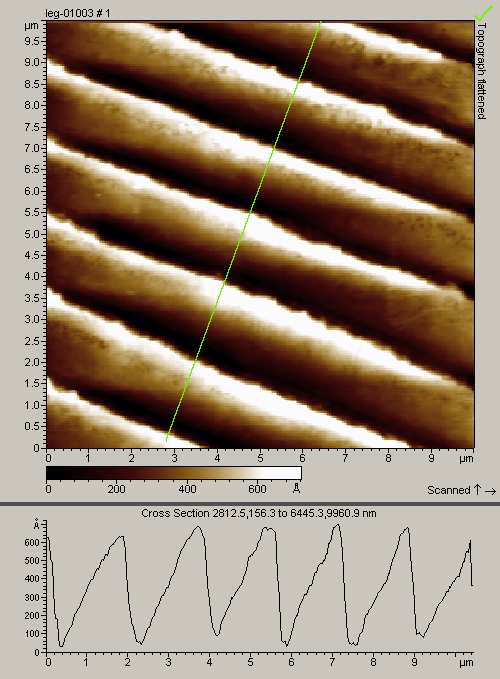
\includegraphics[width=6.5in]{Chapter5/5a_exampleAFM/afm_LEG_xsect1.png} 
   \caption{The Low Energy Grating has a smooth regular profile, shown in this example image measured using an Atomic Force Microprobe (AFM).}
   \label{5a}
\end{figure}

Figure \ref{5a} gives an example of the AFM output, for the LEG grating.  We present  groove profiles for all the gratings starting in Section \ref{gratingResults}, alongside a discussion of their effective diffraction performance.

\section{Diffractometer measurements of actual grating efficiency}
To measure the actual grating efficiency, we used the reflectometer on the Calibration and Standards Beamline (6.3.2) at the Advanced Light Source.  This beamline was designed specifically for testing the reflectivity of soft x-ray optical components like mirrors, thin films, multilayer coatings, and gratings.  It consists of a bending magnet source, a VLS-PGM monochromator with a resolving power of 7000 (Figure \ref{5b-a}), a higher-order suppressor, and a two-circle reflectometer (Figure \ref{5b}).  The beamline optics can focus the monochromator light to a small spot on the sample, or focus at infinite to generate parallel light (TODO REF http://ieeexplore.ieee.org/xpl/freeabs\_all.jsp?arnumber=4994440).

\begin{figure}[htbp] %  figure placement: here, top, bottom, or page
   \centering
   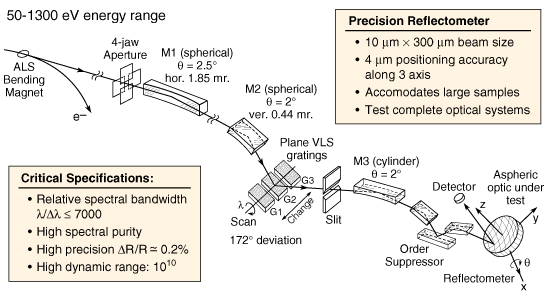
\includegraphics[scale=0.8]{Chapter5/5b_diffractometer/beamlineSchematic2.png} 
   \caption{The Calibration and Standards beamline (6.3.2) at the Advanced Light Source consists of a bending magnet source, a VLS-PGM monochromator with three selectable gratings, a higher-order suppressor, and a two-circle reflectometer shown in more detail in Figure \ref{5b}.  The curvature of refocussing mirror M3 can be adjusted to image the exit slit onto the sample, or to focus the light at infinite.  \textbf{Image from}: (TODO REF http://cxro.lbl.gov/als632/)}
   \label{5b-a}
\end{figure}

\subsection{Beamline 6.3.2 Reflectometer}

\begin{figure}[htbp] %  figure placement: here, top, bottom, or page
   \centering
   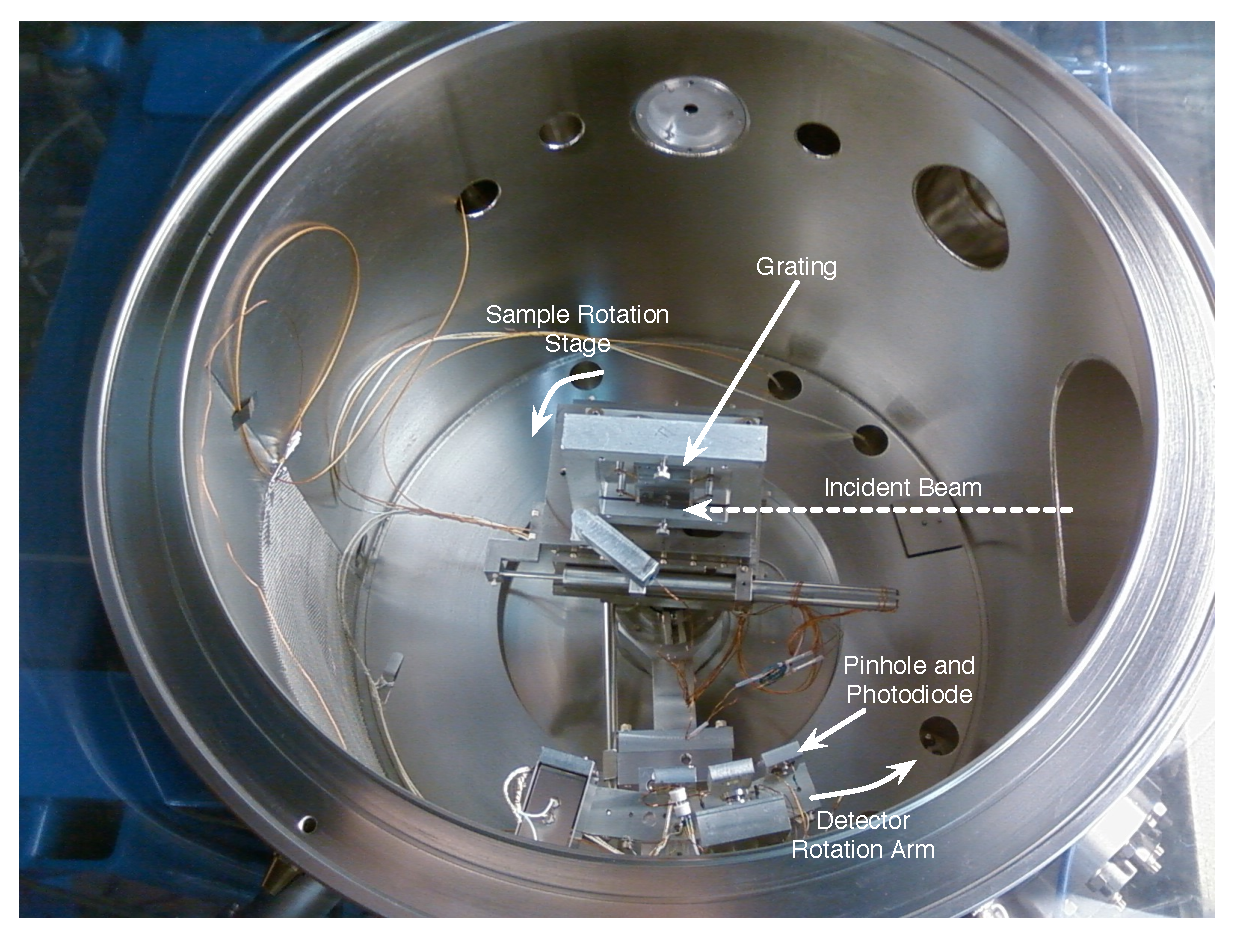
\includegraphics[scale=0.8]{Chapter5/5b_diffractometer/diffractometerLabelled2.pdf} 
   \caption{The reflectometer on Beamline 6.3.2 at the Advanced Light Source allows for independently setting the angle of the gratings in the beam, and setting the angle of a pinhole photodiode detector.  Upstream, filters in the beamline are used to remove contamination from the higher-order light of the monochromator. }
   \label{5b}
\end{figure}

The purpose of the reflectometer endstation (Figure \ref{5b}) is to measure the intensity of light reflected off a sample -- in our case, a grating -- as a function of both incidence and reflection angle.  We used it to determine grating efficiency by positioning the grating at the intended incidence angle relative to the incoming beam,  measuring the intensity at the angle of the outgoing order, and comparing this to the initial beam intensity.  Upstream, the monochromator and order suppressor were used to produce the monochromatic incident beam and set its energy for each datapoint.

In the reflectometer mechanics, a ``two-circle goniometer'' provided independent control over the angle of the sample and the angle of the detector arm, as well as providing precise (4 um) positioning to align the sample in $x$, $y$, and $z$.  The sample holder could accommodate samples up to 200 mm in diameter, which allowed us to mount two of our gratings side-by-side at once.  The detector arm contained a photodiode, a channel electron multiplier (CEM), and a CCD camera; for our grating measurements, we used the photodiode covered by a 2 mm pinhole.

\subsubsection{Diffraction Experiment Procedure}

\begin{enumerate}
\item \textbf{Grating Alignment}\\
To achieve the correct incidence angle and detector angle using the motion control system, the grating had to be aligned correctly.  In the $z$-direction (vertical direction, normal to the grating surface when at grazing incidence), the centre of the grating surface had to coincide with the centre of sample rotation, which was also at the height of the beam.  In the $x$-direction (parallel to the grating grooves), the beam had to land on the centre of the grating; otherwise the curvature of the grating would introduce a slope in the saggital direction, and we would end up with conical mounting.
	\begin{enumerate}
	\item To crudely align the grating in the $z$-direction, the grating angle was set to zero degrees, and the CCD camera was placed at a detection angle of 0 degrees.  With the sample moved fully down out of the way in $z$, this allowed the beam to shine past the grating directly onto the centre of the CCD, confirming the alignment of the beam angle. 
	\item The grating was then moved upward in $z$ until it just started blocking the beam from reaching the CCD detector, indicating that the surface was now at (or just above) beam height.
	\item With the grating blocking the CCD detector in this position, it was translated in $x$ until light returned, indicating that the beam had fallen off the side edge of the grating.  This was repeated in the $(-x)$-direction, providing us with the position of the opposite side; the grating was then positioned midway between these two positions, achieving alignment in $x$.
	\item To accurately complete the alignment in $z$, the grating was angled at two degrees, and the photodiode detector was positioned to collect reflected (0th order) light at four degrees.  As long as the beam was incident on the grating, this would register a signal on the detector.  The grating was then translated upward in $z$ until the signal disappeared, indicating that the beam had fallen off the bottom edge of the grating. This $z$-position was recorded as the bottom grating edge.
	\item The grating was then lowered in $z$ until the signal disappeared again, indicating that the beam had fallen off the top edge of the grating.  This $z$-position was recorded as the top grating edge, and then the grating was moved to the average of the two recorded $z$-positions; this process ensured that the beam was now incident on the exact centre of the grating.
	\end{enumerate}
	
\item \textbf{Scanning Modes}\\
All of the efficiency plots we calculated in Chapter 5 to predict the REIXS gratings' performance show efficiency as a function of photon energy.  We wanted to show our real-world measurements in the same format, which required us to scan the beamline energy while measuring the intensity of the desired order with the photodiode.  Therefore, the detector angle had to change as we changed the beamline energy, according to the outgoing angle specified by the grating equation (Equation \ref{gratingEquation}).  

If we had known the groove density very accurately, we could have calculated the correct detector angle and positioned the detector simultaneously while scanning the beamline energy.  However, for brand new gratings, it would be unlikely for the groove density to end up exactly as requested from the manufacturer; in this case we would actually need to conduct a two-dimensional scan: for every photon energy datapoint, we would need to conduct an angular scan of the photodiode to find the diffraction peaks.\footnote{After completing this scan, we could use the angular position of the diffraction peaks to calculate the actual groove density, but only within a precision determined by the angular extent of the 2mm photodiode pinhole.}

For four of the gratings, we did have an accurate groove density, obtained from Power Spectral Density (PSD) measurements taken by the metrology lab at the Canadian Light Source.  However, for two of the gratings, the exact groove density was unknown, so we had to use the two-dimensional scan method.  Mechanically, this is actually the simplest way to operate the reflectometer, and an example of the results are shown in Figure \ref{5c}.  The procedure was as follows:

	\begin{enumerate}
	\item The monochromator was set to the desired photon energy, and the corresponding filters were selected in the higher-order absorber.
	\item The grating was positioned at its specified incidence angle relative to the beam, as it would be during operation of the spectrometer.
	\item The photodiode was scanned, recording intensity as a function of outgoing angle.
	\item The grating was moved out of the way of the beam, and the photodiode was placed at zero degrees to measure the direct beam intensity; this intensity value was used to normalize the data as described in Item \ref{normalizationEff}. 
	\item The results (Figure \ref{5c}) show the intensity of reflected light as a fraction of the incident beam intensity, as a function of detector angle.  The 0th order, 1st order, and 2nd order peaks are clearly seen; we can quickly check that the 0th order peaks show no wavelength dependency and occur at twice the incidence angle.  The grating efficiency in the $n$th order is taken from the height at the centre of the $n$th diffraction peak.
	\end{enumerate}

This procedure had to be repeated every photon energy datapoint that we wanted to test, and this could be tedious.  For the gratings where the groove density was known accurately, we used a more expedient method, which required synchronized scanning of the detector angle and beamline energy:

	\begin{enumerate}
	\item The higher-order suppressor was configured for the energy range of the scan. (This limited each individual scan to the valid energy range of a single higher-order filter; see Section \ref{higherOrderContamination})
	\item The control software was configured to move the detector angle in tandem with the beamline energy to stay on top of the diffraction peak, using the grating equation and the specified groove density and order.
	\item The beamline energy and the detector angle were scanned together, recording the intensity of the diffracted order at each datapoint.
	\item The grating was then moved out of the way of the beam, and the detector angle was set to zero degrees to measure the direct beam.  The beamline energy scan was repeated to measure the incident intensity as a function of energy, to use for normalization (see Item \ref{normalizationEff}).
	\item The normalized results (Figure \ref{5d}) directly show the intensity of diffracted light in the specified order as a fraction of the incident beam intensity, as a function of energy .  With this method, it is easier to measure a finely-spaced set of datapoints along the energy axis, to compare with our efficiency prediction plots in Chapter 5.
	\end{enumerate}

\item Wavelength Calibration
\item Normalization
\label{normalizationEff}
\end{enumerate}

\begin{figure}[htbp] %  figure placement: here, top, bottom, or page
   \centering
   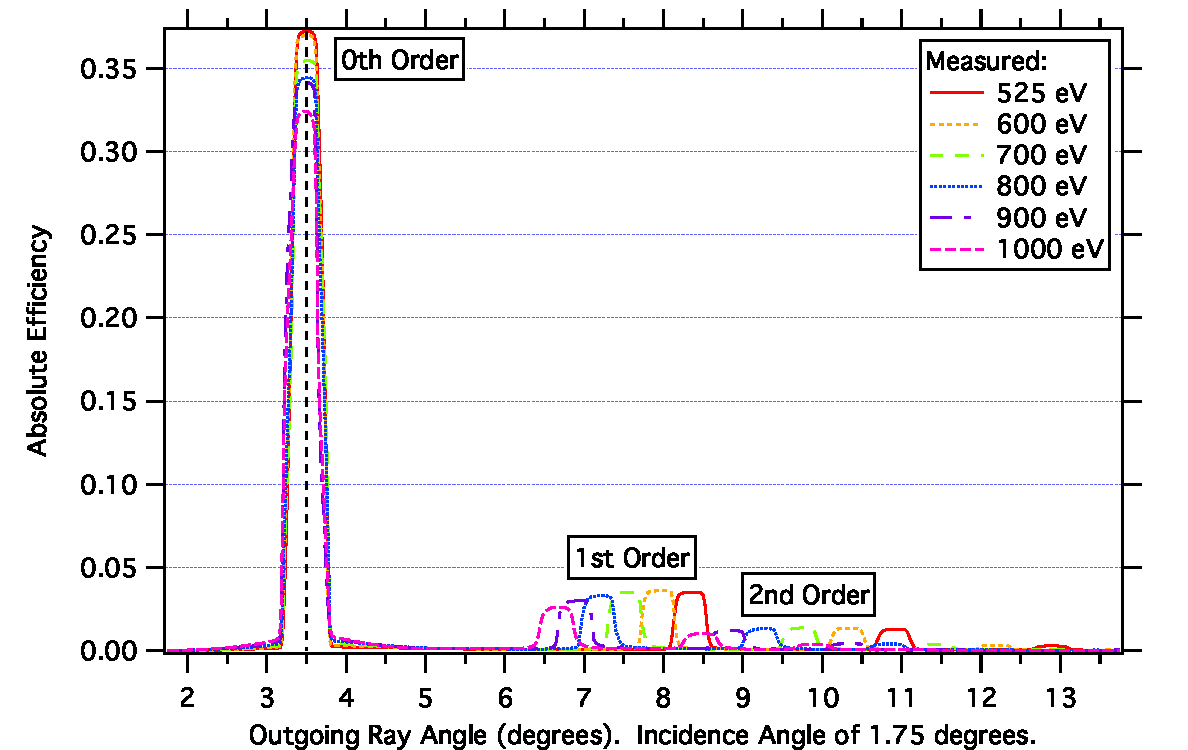
\includegraphics[scale=0.8]{Chapter5/5c_angleScan/5c.pdf} 
   \caption{The simplest diffractometer experiment scans the detector angle while illuminating the grating with a constant photon energy.  The diffraction orders are visible as peaks along the outgoing angle axis (here, measured up from the grating surface at 0$\deg$).  The 0th order (reflection) peak is easily visible at 3.5$\deg$, or twice the incident angle (88.25$\deg$, or 1.75$\deg$ from grazing).  Grating: HRHEG.}
   \label{5c}
\end{figure}

\begin{figure}[htbp] %  figure placement: here, top, bottom, or page
   \centering
   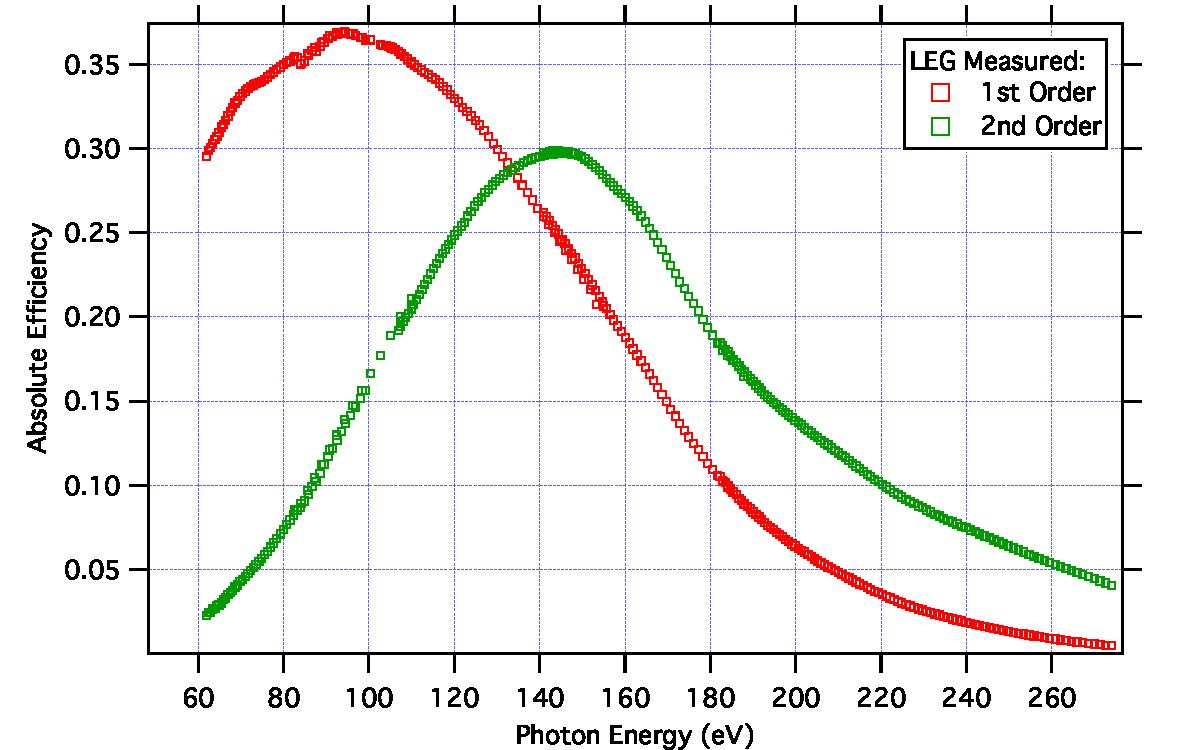
\includegraphics[scale=0.8]{Chapter5/5d_energyScan/5d_LEG.pdf} 
   \caption{When the groove density of a grating is accurately known, the detector angle can be moved in tandem with the beamline energy to keep it on the diffraction peak as the incident photon energy is scanned.  This allows faster, nearly continuous efficiency measurements as a function of photon energy.  Grating: LEG}
   \label{5d}
\end{figure}

\subsubsection{Sources of Error}
\label{higherOrderContamination}
\begin{enumerate}
\item - higher order contamination
\item - monochromator energy calibration
\item - photodiode dark current (depends on temperature)
\item - energy dispersion across detector pinhole (finite size of pinhole + finite resolution dE)
\item - defocussing ?
\item - grating rotation (saggital)
\item - only testing a spot size in the middle of the grating, 0.01mm x 0.3mm
\end{enumerate}

- mono: higher-order light contamination.  Uses filters in front of end station

\section{Real-world grating effects}
\label{realWorldEffects}
\subsection{Stray Radiant Energy}
http://gratings.newport.com/information/technotes/technote9.asp
\subsubsection{Surface roughness}
 (scattering: uniform decrease in efficiency)
  Other way to think about: periodic structures with \emph{many} frequency components. Diffract all over the place.
  
  TODO: Find reference and descriptive math...
  
          - Not modelled.  Accept a uniform constant reduction (usually about ~50\%) lower due to scattering.

\begin{figure}[htbp] %  figure placement: here, top, bottom, or page
   \centering
   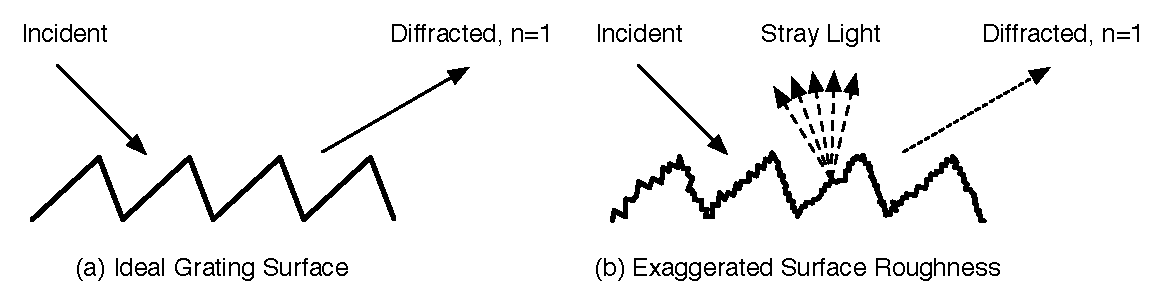
\includegraphics[scale=0.8]{Chapter5/5e_surfaceRoughness/5e.pdf} 
   \caption{Roughness of the grating surface scatters stray light outside the diffraction orders}
   \label{5e}
\end{figure}
       

\subsubsection{Dust, scratches, pinholes act as scattering centers}
\subsubsection{Irregularities in the groove position create ghost peaks}
\subsubsection{Irregularities along the groove direct light elsewhere}
reflect off axis... reduce periodicity... disrupt the perfect grating model. May be directed or diffuse.
\subsection{Blaze angle errors shift the efficiency peak}
\subsection{Coating oxidation changes the reflectivity spectrum}

\begin{figure}[htbp] %  figure placement: here, top, bottom, or page
   \centering
   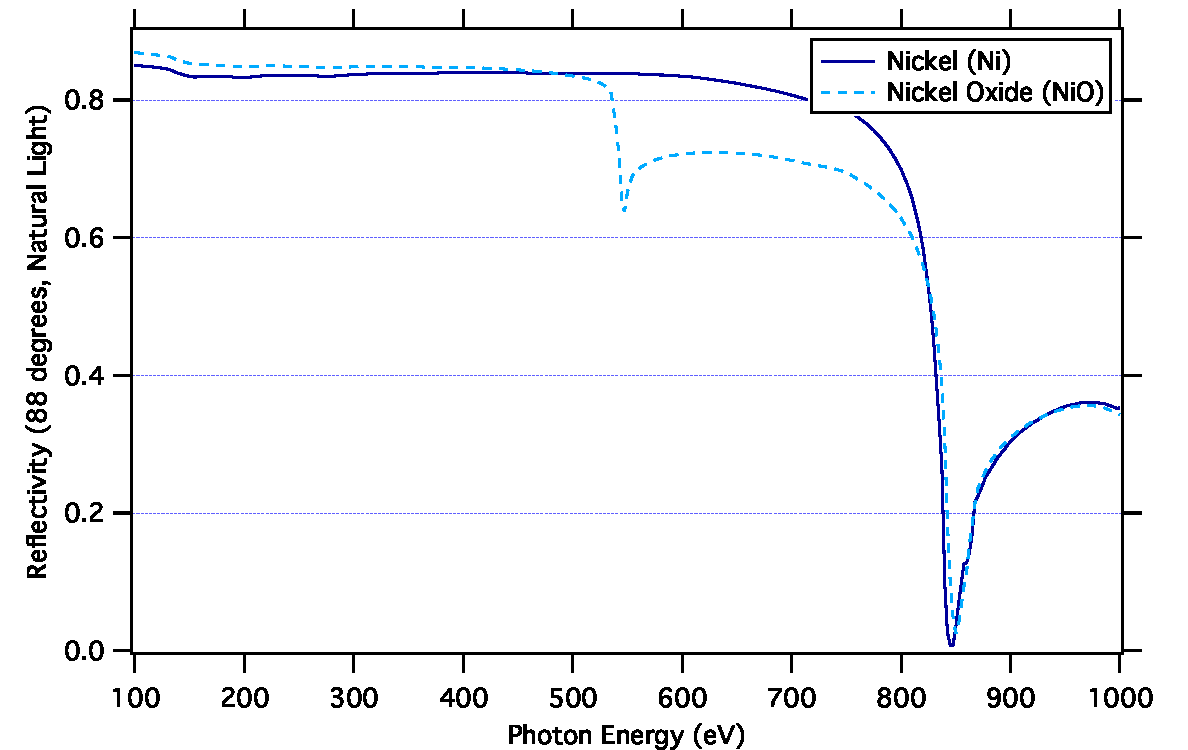
\includegraphics[scale=0.8]{Chapter5/5f_oxidized/Ni_NiO_reflec.pdf} 
   \caption{Unprotected Nickel quickly forms a surface oxide of NiO, which strongly reduces the reflectivity at the Oxygen edge (525eV) }
   \label{5f}
\end{figure}

\section{Grating results}
\label{gratingResults}
   : (and comparison to theoretical)
\subsection{LEG} (gold): profile clean; as expected; blaze angle off. [modelled]

\begin{figure}[htbp] %  figure placement: here, top, bottom, or page
   \centering
   \includegraphics[scale=0.8]{Chapter5/5y_afm/LEG.pdf} 
   \caption{AFM measurements of the Low Energy Grating (LEG) profile, averaged along the grooves (TODO um x TODO um).  The best-fit blaze angle is at the centre of the grating.}
   \label{5y-leg}
\end{figure}

\begin{figure}[htbp] %  figure placement: here, top, bottom, or page
   \centering
   \includegraphics[scale=0.8]{Chapter5/5x_comparison/LEG.pdf} 
   \caption{Theoretical and measured efficiency of the Low Energy Grating (LEG).}
   \label{5x-leg}
\end{figure}


\subsection{IMP} (nickel): Profile clean, blaze angle off [modelled].  Oxidized� Modelled as NI, layer of NiO.

TEST: NiO on top of Ni? layer thickness
Caveat: Henke data reflectivities are not correct at/near absorption edges... shouldn't totally match theoretical shape.

          - compare AFM and fitted
          
          scattering factor: http://www2.astro.psu.edu/~niel/astro485/xrayschool/schwartz-xray\_optics.pdf --> 1/sin(theta)

\begin{figure}[htbp] %  figure placement: here, top, bottom, or page
   \centering
   \includegraphics[scale=0.8]{Chapter5/5y_afm/IMP.pdf} 
   \caption{AFM measurements of the Impurity Grating (IMP) profile, averaged along the grooves (TODO um x TODO um).  The best-fit blaze angle is at the centre of the grating.}
   \label{5y-imp}
\end{figure}

\begin{figure}[htbp] %  figure placement: here, top, bottom, or page
   \centering
   \includegraphics[scale=0.8]{Chapter5/5x_comparison/IMP.pdf} 
   \caption{Theoretical and measured efficiency of the Impurity Grating (IMP).}
   \label{5x-imp}
\end{figure}


\subsection{MEG} (nickel): profile ok, blaze angle off [modelled].  Oxidized� Modelled as combination of NiO and NiO2.

\begin{figure}[htbp] %  figure placement: here, top, bottom, or page
   \centering
   \includegraphics[scale=0.8]{Chapter5/5y_afm/MEG.pdf} 
   \caption{AFM measurements of the Medium Energy Grating (MEG) profile, averaged along the grooves (TODO um x TODO um).  The best-fit blaze angle is at the centre of the grating.}
   \label{5y-meg}
\end{figure}

\begin{figure}[htbp] %  figure placement: here, top, bottom, or page
   \centering
   \includegraphics[scale=0.8]{Chapter5/5x_comparison/MEG.pdf} 
   \caption{Theoretical and measured efficiency of the Medium Energy Grating (LEG).}
   \label{5x-meg}
\end{figure}

\subsection{HEG} (Pt): almost no diffraction performance at all. AFM: revealed double-peak structure; not ruled correctly. Sent back to manuf.

\begin{figure}[htbp] %  figure placement: here, top, bottom, or page
   \centering
   \includegraphics[scale=0.8]{Chapter5/5y_afm/HEG.pdf} 
   \caption{AFM measurements of the High Energy Grating (HEG) profile, averaged along the grooves (TODO um x TODO um).  Severe ruling errors were apparent.  The profile wasn't sufficiently triangular to attempt to fit a blaze angle.}
   \label{5y-heg}
\end{figure}

\begin{figure}[htbp] %  figure placement: here, top, bottom, or page
   \centering
   \includegraphics[scale=0.8]{Chapter5/5x_comparison/HEG.pdf} 
   \caption{Theoretical and measured efficiency of the High Energy Grating (LEG).}
   \label{5x-heg}
\end{figure}

\subsection{HRMEG and HRHEG}

\begin{figure}[htbp] %  figure placement: here, top, bottom, or page
   \centering
   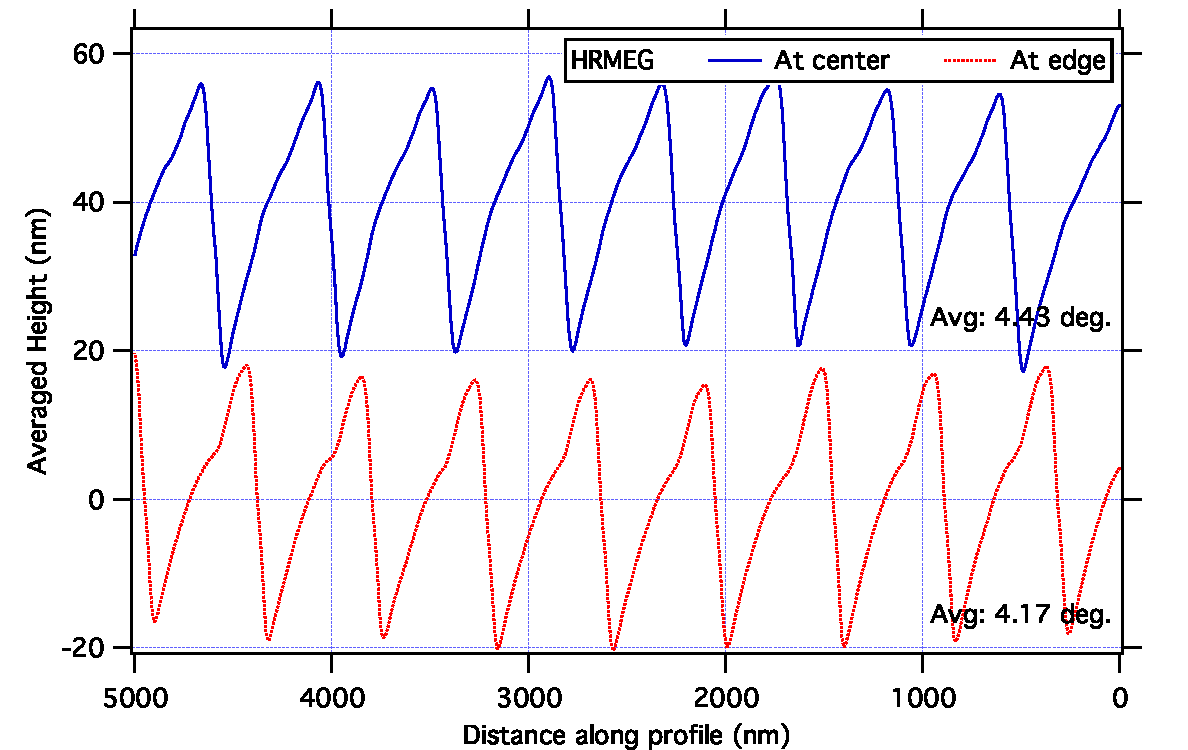
\includegraphics[scale=0.8]{Chapter5/5y_afm/HRMEG.pdf} 
   \caption{AFM measurements of the HighRes Medium Energy Grating (HRMEG) profile, averaged along the grooves (TODO um x TODO um).  The best-fit blaze angle is at the centre of the grating.}
   \label{5y-hrmeg}
\end{figure}

\begin{figure}[htbp] %  figure placement: here, top, bottom, or page
   \centering
   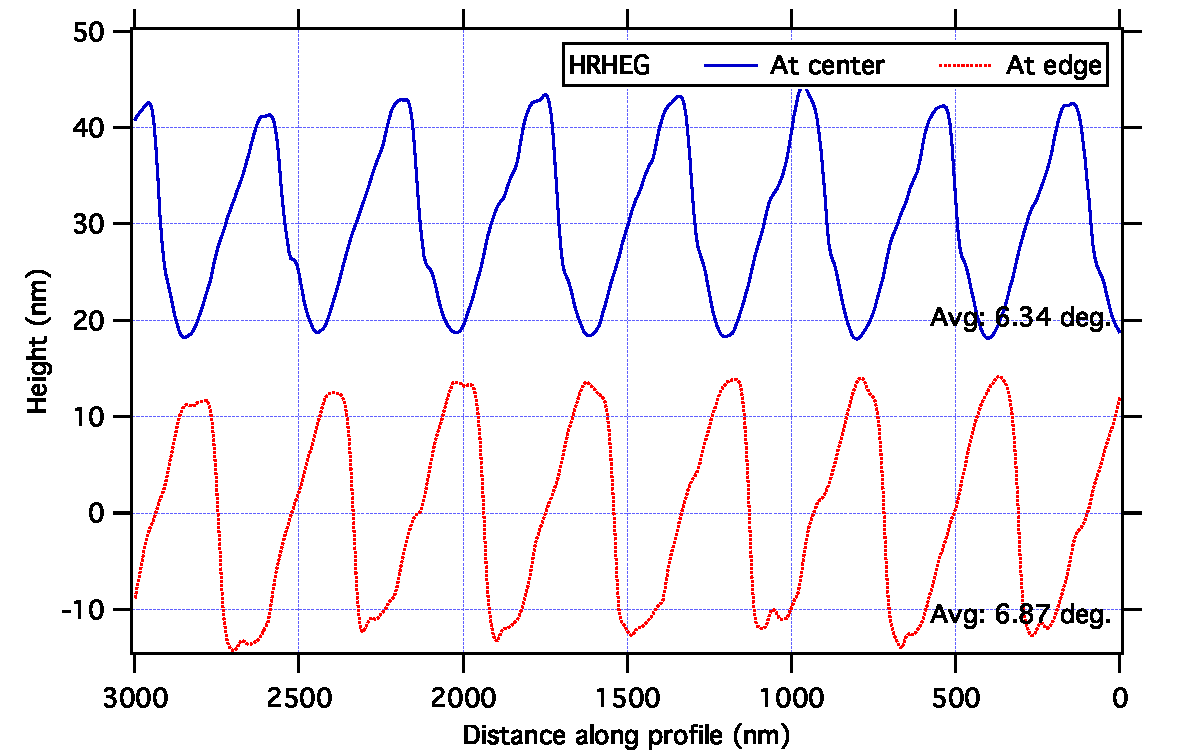
\includegraphics[scale=0.8]{Chapter5/5y_afm/HRHEG.pdf} 
   \caption{AFM measurements of the HighRes High Energy Grating (HRHEG) profile, averaged along the grooves (TODO um x TODO um).  The best-fit blaze angle is at the centre of the grating.}
   \label{5y-hrheg}
\end{figure}




 (Pt): blaze angles very off� Unsuitable for actual application in 3rd order.
          - Temporary plan: Using HRHEG (2600l/mm) in place of HEG (2000l/mm) since blaze angle error makes it suitable for use in 1st order.
               - DATA 5q: plot expected reduction in efficiency
               
